\documentclass[10pt,twocolumn,letterpaper]{article}
\usepackage[rebuttal]{cvpr}

% Include other packages here, before hyperref.
\usepackage{graphicx}
\usepackage{amsmath}
\usepackage{amssymb}
\usepackage{booktabs}
\usepackage{url}
\usepackage{enumitem}
\usepackage{caption}
\captionsetup{skip=2pt}
\usepackage{wrapfig}
\usepackage{float}

% If you comment hyperref and then uncomment it, you should delete
% egpaper.aux before re-running latex.  (Or just hit 'q' on the first latex
% run, let it finish, and you should be clear).
\usepackage[pagebackref,breaklinks,colorlinks,bookmarks=false]{hyperref}

% Support for easy cross-referencing
\usepackage[capitalize]{cleveref}
\crefname{section}{Sec.}{Secs.}
\Crefname{section}{Section}{Sections}
\Crefname{table}{Table}{Tables}
\crefname{table}{Tab.}{Tabs.}

% If you wish to avoid re-using figure, table, and equation numbers from
% the main paper, please uncomment the following and change the numbers
% appropriately.
%\setcounter{figure}{2}
%\setcounter{table}{1}
%\setcounter{equation}{2}

% If you wish to avoid re-using reference numbers from the main paper,
% please uncomment the following and change the counter for `enumiv' to
% the number of references you have in the main paper (here, 6).
%\let\oldthebibliography=\thebibliography
%\let\oldendthebibliography=\endthebibliography
%\renewenvironment{thebibliography}[1]{%
%     \oldthebibliography{#1}%
%     \setcounter{enumiv}{6}%
%}{\oldendthebibliography}


%%%%%%%%% COMP 472 - Project  - PLEASE UPDATE
\def\cvprPaperID{Classification of MRI images for brain tumor diagnosis} % *** Enter the CVPR Paper ID here
\def\confName{Project Proposal}
\def\confYear{2026}

\begin{document}

%%%%%%%%% COMP 472 - Project Proposal- PLEASE UPDATE
\title{Classification of MRI images for brain tumor diagnosis}  % **** Enter the paper title here


\maketitle
\thispagestyle{empty}
\appendix

%%%%%%%%% BODY TEXT - ENTER YOUR RESPONSE BELOW
%-------------------------------------------------------------------------
\textbf{Problem Statement and Application.} Our team has selected the detection and classification of various brain tumor types from MRI images for our project. We aim to evaluate the strengths and weaknesses of various Convolutional Neural Network (CNN) architectures in identifying brain tumors. Although MRI technology is extremely effective at imaging brain tumors\cite{mri}, automated tumor classification presents several computational challenges. MRI scans exhibit significant variability in contrast, resolution, and acquisition protocols\cite{mri_variability}, which affects feature consistency across samples. Moreover, different tumor types often share similar visual characteristics, making inter-class discrimination difficult. The task is further complicated by class imbalance, limited dataset sizes for certain tumor categories, and intra-class variability in tumor shape, size, and location. These factors make brain tumor classification a demanding problem, requiring robust CNN architectures capable of learning discriminative features despite data heterogeneity and subtle visual differences.

%------------------------------------------------------------------------
\textbf{Image Dataset Selection.} We selected three publicly available brain MRI image datasets that differ in size and number of classes to enable a progressive evaluation of CNN architectures.
\begin{table}[h]
	\vspace{-4mm}
	\centering
	\small
	\setlength{\tabcolsep}{3pt}
	\renewcommand{\arraystretch}{0.9}
	\begin{tabular}{|l|c|c|c|c|}
		\hline
		Dataset & Imgs & Classes & Imgs/Classes & Size \\
		\hline
		1\cite{dataset1} & 3264 & 4 & 826/822/395/827 & Mixed, max630×630 \\
		\hline
		2\cite{dataset2} & 7023 & 4 & 1321/1339/1595/1457 & 512×512 \\
		\hline
		3\cite{dataset3} & 4478 & 44 & 17--272 & Mixed, max630×630 \\
		\hline
	\end{tabular}
	\caption{Dataset overview}
	\vspace{-4mm}
\end{table}
The first dataset, Brain Tumor Classification (MRI)\cite{dataset1}, and the second dataset, Brain Tumor MRI Dataset\cite{dataset2}, both categorize images into 4 classes (Glioma, Meningioma, Pituitary tumor, and No Tumor), providing meaningful common brain tumor categories\cite{commonbraintumor} with varying image quantities. While the first dataset contains a limited number of images, the second offers more than double the volume, enabling us to examine how CNN models perform with identical class structures but different dataset sizes.
 \begin{wrapfigure}{l}{0.40\columnwidth}  % r = right side, l = left side
 	\vspace{-14pt}
	\centering
	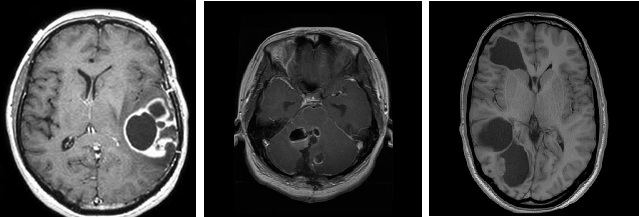
\includegraphics[width=0.45\columnwidth]{datasetcomparison.jpg}
	\caption{Comparison of dataset images}
	\label{fig:yourlabel}
	\vspace{-12pt}
\end{wrapfigure} 
 The third dataset\cite{dataset3}, despite having fewer total images ,introduces a higher class diversity with 44 different types of brain tumors, lesions, and normal brain tissue to compare. Each were captured using different MRI sequences, which significantly raises the classification difficulty. This progression from a small 4-class dataset, to a larger 4-class dataset, to a medium-sized highly fine-grained 44-class dataset creates a controlled framework to analyze how CNN models of different capacities perform as dataset scale and class granularity change.


%-------------------------------------------------------------------------
\textbf{Possible Methodology.}Given the datasets come from different sources and vary in size, format and image resolution, we preprocess them into a standardized format. To prevent overfitting due to the small size of the available datasets, we apply data augmentation techniques to  increase the number of images used to train the model by transforming the dataset's images.\cite{dataaugment} These transformation includes geometric transformations such as small rotations, cropping, zooming in , and color space transformations like changing brightness.\cite{datacamp_augmentation}
Since we are using PyTorch for this project, all of our images will need to be converted into tensors of the same size 224x224 and dimension.


The choices in CNN architectures allow us to observe how different models perform depending on their size and the complexity of their datasets, while also ensuring that the models can be trained within the computational resources of average GPUs. MobileNet V2\cite{mobilenet} is a lightweight architecture design for low-resource environments, making it ideal for evaluating the performance of compact models on medical imaging. ResNet-34\cite{resnet} is a larger architecture that enables stable training thanks to its residual connections. EfficientNet-B2\cite{efficientnet} is medium sized compared to the aforementioned architectures. We can expect the three CNN architectures to show varying levels of performance depending on the dataset’s complexity. Since MobileNet V2 is the lightest model, it is expected to train quickly on the smallest dataset, but may struggle with the biggest dataset due to its limited capacity. ResNet-34 could provide a solid balance between accuracy and computational cost, likely outperforming MobileNet on the larger datasets. Despite EfficentNet-B2 being lighter than ResNet in terms of FLOPs and parameter counts, it uses a compound scaling strategy to balance depth, width and resolution, and should therefore offer the best overall performance.
By studying how model capacity, dataset complexity, and transfer learning influence performance, this project could help identify which architectures are best suited for MRI-based tumor classification given different resource constraints. This research could guide the design of more reliable diagnostic tools and showcase the trade-offs between lightweight and larger architectures.

Model performance will be evaluated using several metrics.\cite{modelmetrics} Accuracy measures the proportion of correct predictions across all classes. Precision measures how often predictions for a specific class are correct, catching false positives, while recall measures how many actual class members are identified, catching false negatives. The F1-score quantifies the balance between precision and recall. Mean Average Precision assesses whether a model is consistently correct about each given class, which is especially helpful for datasets with multiple classes where accuracy alone is less informative due to less detectable or rarer classes. Loss curves track the inaccuracy of a model over time to observe the learning rate across its training.\newpage


\newpage
%------------------------------------------------------------------------
\noindent\textbf{Project Gantt Chart} \\
\noindent\href{https://1drv.ms/i/c/245f806ee8e62c91/IQDAWdYL6_TwTbmw-qErISu8AeUMVQ0f43GwPqAy-swBEaQ?e=i2Yo0U}{Gantt Chart File}

\vspace{10pt}

\begin{center}
	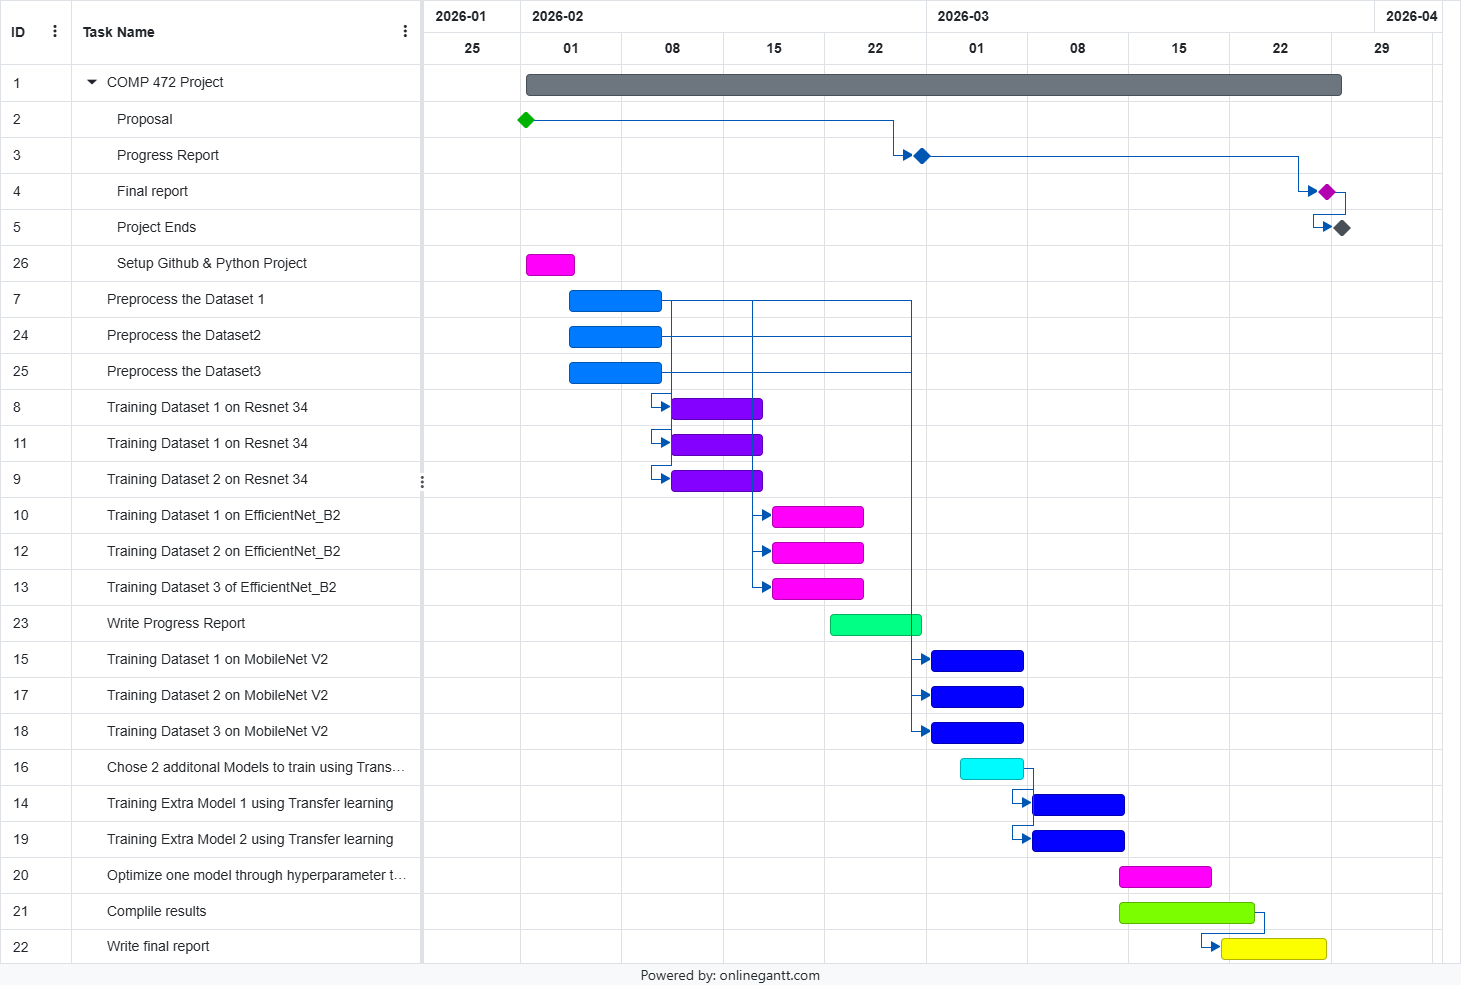
\includegraphics[width=1.00\textwidth]{COMP472_Project_Gantt.png}
	\captionof{figure}{COMP 472 - Group C Project Gantt Chart}
	\label{fig:fullwidth}
	
	\vspace{10pt}
	
	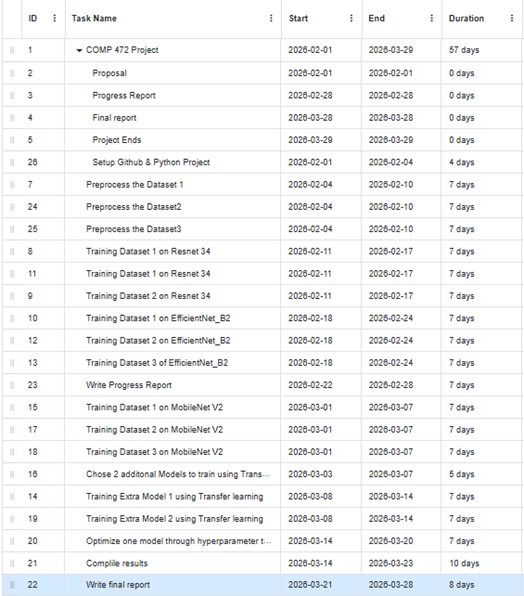
\includegraphics[width=0.60\textwidth]{COMP472_Project_Gantt-2.png}
	\captionof{figure}{COMP 472 - Group C Project Gantt Chart Details}
	\label{fig:fullwidth2}
\end{center}

\clearpage
%%%%%%%%% REFERENCES

   \bibliographystyle{ieeetr}
\bibliography{egbib}


\end{document}
